\section{26 Sep 23 - Activity: Electrostatic
Fields}\label{sep-23---activity-electrostatic-fields}

As we saw the electric field is described by the 4 Maxwell equations.
But, in the electrostatic situation where the charges do not move, we
find the electric field is described by the following equations:

\[\nabla \cdot \mathbf{E} = \frac{\rho}{\epsilon_0}\]

\[\nabla \times \mathbf{E} = 0\]

These linear partial differential equations can be solved analytically
for a number of situations. In this activity we will explore the
electric field for a number of situations.

\subsection{The del operator}\label{the-del-operator}

The del operator (\(\nabla\)) is a differential vector operator that can
act in the same way that vectors do (i.e., through a dot \(\cdot\) or
cross \(\times\) product). In addition, it can operate on a scalar
function to produce a vector function (i.e.,
\(\mathbf{E}(x,y,z) = - \nabla V(x,y,z)\)). The operator itself is given
by:

\[\nabla = \hat{x} \frac{\partial}{\partial x} + \hat{y} \frac{\partial}{\partial y} + \hat{z} \frac{\partial}{\partial z}\]

where \(\hat{x}\), \(\hat{y}\), and \(\hat{z}\) are the unit vectors in
the \(x\), \(y\), and \(z\) directions, respectively. It acts on a
scalar function \(f(x,y,z)\) as follows:

\[\nabla f(x,y,z) = \hat{x} \frac{\partial f}{\partial x} + \hat{y} \frac{\partial f}{\partial y} + \hat{z} \frac{\partial f}{\partial z}\]

When taking the dot product (the divergence) of a vector function
\(\mathbf{F}(x,y,z)\), it acts as follows:

\[\nabla \cdot \mathbf{F}(x,y,z) = \frac{\partial F_x}{\partial x} + \frac{\partial F_y}{\partial y} + \frac{\partial F_z}{\partial z}\]

And finally, when taking the cross product (the curl) of a vector
function \(\mathbf{F}(x,y,z)\), it acts as follows:

\[\nabla \times \mathbf{F}(x,y,z) = \left( \frac{\partial F_z}{\partial y} - \frac{\partial F_y}{\partial z} \right) \hat{x} + \left( \frac{\partial F_x}{\partial z} - \frac{\partial F_z}{\partial x} \right) \hat{y} + \left( \frac{\partial F_y}{\partial x} - \frac{\partial F_x}{\partial y} \right) \hat{z}\]

We rarely make use of the full form of these differential equations,
instead solving them in restricted and highly symmetric cases (e.g.,
using Gauss's Law), computing directly the field contributed by
infinitesimal charges (e.g., using Coulomb's Law), or using numerical
methods (e.g., using summation or other techniques).

Often, the most productive approach tends to be using electric potential
(a scalar function), which we will discuss later.

\begin{Shaded}
\begin{Highlighting}[]
\CommentTok{\#\# run to import libraries}
\ImportTok{import}\NormalTok{ numpy }\ImportTok{as}\NormalTok{ np}
\ImportTok{import}\NormalTok{ matplotlib.pyplot }\ImportTok{as}\NormalTok{ plt}
\ImportTok{from}\NormalTok{ matplotlib.colors }\ImportTok{import}\NormalTok{ Normalize}
\ImportTok{import}\NormalTok{ matplotlib.cm }\ImportTok{as}\NormalTok{ cm}
\end{Highlighting}
\end{Shaded}

\subsection{Coulomb's Law and the Electric
Field}\label{coulombs-law-and-the-electric-field}

As you have encountered in the past, a generic expression for the
electric field observed at location \(\mathbf{r}\) due to a point charge
\(q\) at location \(\mathbf{r}'\) is given by:

\[\mathbf{E} = \dfrac{q}{4\pi\epsilon_0} \dfrac{\mathbf{r} - \mathbf{r}'}{\left|\mathbf{r} - \mathbf{r}'\right|^3}\]

Notice that the electric field is a vector function of position and the
differences that appear are vector ones:

\[\mathbf{r} - \mathbf{r}' = (x-x')\hat{x} + (y-y')\hat{y} + (z-z')\hat{z}\]

We can show that the general solution for the electric field due to a
set of point charges is simply the
\href{https://en.wikipedia.org/wiki/Superposition_principle}{superposition}
of the individual fields due to each charge:

\[\mathbf{E} = \sum_i \mathbf{E}_i = \sum_i \dfrac{q_i}{4\pi\epsilon_0} \dfrac{\mathbf{r} - \mathbf{r}_i}{\left|\mathbf{r} - \mathbf{r}_i\right|^3}\]

where \(\mathbf{E}_i\) is the electric field due to the ith charge.

\subsubsection{Visualization of the Electric
Field}\label{visualization-of-the-electric-field}

Below we have written a a function that computes the electric field for
a point charge at a known location. We use a few different libraries and
known functions that we have used in the past for dynamical systems. But
we apply them to the electric field.

\begin{Shaded}
\begin{Highlighting}[]

\KeywordTok{def}\NormalTok{ electric\_field(charge, x\_points, y\_points, x\_charge}\OperatorTok{=}\DecValTok{0}\NormalTok{, y\_charge}\OperatorTok{=}\DecValTok{0}\NormalTok{):}
\NormalTok{    k }\OperatorTok{=} \FloatTok{8.99e9}  \CommentTok{\# Nm\^{}2/C\^{}2, Coulomb\textquotesingle{}s constant}
    
    \CommentTok{\# Initialize electric field components to zero}
\NormalTok{    E\_x }\OperatorTok{=}\NormalTok{ np.zeros\_like(x\_points)}
\NormalTok{    E\_y }\OperatorTok{=}\NormalTok{ np.zeros\_like(y\_points)}
    
    \CommentTok{\# Calculate electric field components due to the point charge at each point on the grid}
    \ControlFlowTok{for}\NormalTok{ i }\KeywordTok{in} \BuiltInTok{range}\NormalTok{(x\_points.shape[}\DecValTok{0}\NormalTok{]):}
        \ControlFlowTok{for}\NormalTok{ j }\KeywordTok{in} \BuiltInTok{range}\NormalTok{(y\_points.shape[}\DecValTok{1}\NormalTok{]):}
\NormalTok{            r\_x }\OperatorTok{=}\NormalTok{ x\_points[i, j] }\OperatorTok{{-}}\NormalTok{ x\_charge}
\NormalTok{            r\_y }\OperatorTok{=}\NormalTok{ y\_points[i, j] }\OperatorTok{{-}}\NormalTok{ y\_charge}
\NormalTok{            r\_magnitude }\OperatorTok{=}\NormalTok{ np.sqrt(r\_x}\OperatorTok{**}\DecValTok{2} \OperatorTok{+}\NormalTok{ r\_y}\OperatorTok{**}\DecValTok{2}\NormalTok{)}
            \ControlFlowTok{if}\NormalTok{ r\_magnitude }\OperatorTok{!=} \DecValTok{0}\NormalTok{:  }\CommentTok{\# Avoid division by zero}
\NormalTok{                r\_unit\_x }\OperatorTok{=}\NormalTok{ r\_x }\OperatorTok{/}\NormalTok{ r\_magnitude}
\NormalTok{                r\_unit\_y }\OperatorTok{=}\NormalTok{ r\_y }\OperatorTok{/}\NormalTok{ r\_magnitude}
\NormalTok{                E\_x[i, j] }\OperatorTok{=}\NormalTok{ k }\OperatorTok{*}\NormalTok{ charge }\OperatorTok{*}\NormalTok{ r\_unit\_x }\OperatorTok{/}\NormalTok{ r\_magnitude}\OperatorTok{**}\DecValTok{2}
\NormalTok{                E\_y[i, j] }\OperatorTok{=}\NormalTok{ k }\OperatorTok{*}\NormalTok{ charge }\OperatorTok{*}\NormalTok{ r\_unit\_y }\OperatorTok{/}\NormalTok{ r\_magnitude}\OperatorTok{**}\DecValTok{2}
    
    \ControlFlowTok{return}\NormalTok{ E\_x, E\_y}

\KeywordTok{def}\NormalTok{ plot\_electric\_field(X, Y, E\_x, E\_y, stream\_color}\OperatorTok{=}\StringTok{\textquotesingle{}b\textquotesingle{}}\NormalTok{):}
\NormalTok{    fig, axs }\OperatorTok{=}\NormalTok{ plt.subplots(}\DecValTok{1}\NormalTok{, }\DecValTok{3}\NormalTok{, figsize}\OperatorTok{=}\NormalTok{(}\DecValTok{15}\NormalTok{, }\DecValTok{5}\NormalTok{))}
    
    \CommentTok{\# First Subplot {-} Quiver Plot}
\NormalTok{    axs[}\DecValTok{0}\NormalTok{].quiver(X, Y, E\_x, E\_y, scale}\OperatorTok{=}\FloatTok{1e6}\NormalTok{, color}\OperatorTok{=}\StringTok{\textquotesingle{}r\textquotesingle{}}\NormalTok{)}
\NormalTok{    axs[}\DecValTok{0}\NormalTok{].set\_title(}\StringTok{\textquotesingle{}Quiver Plot\textquotesingle{}}\NormalTok{)}
\NormalTok{    axs[}\DecValTok{0}\NormalTok{].set\_xlabel(}\StringTok{\textquotesingle{}x [m]\textquotesingle{}}\NormalTok{)}
\NormalTok{    axs[}\DecValTok{0}\NormalTok{].set\_ylabel(}\StringTok{\textquotesingle{}y [m]\textquotesingle{}}\NormalTok{)}
\NormalTok{    axs[}\DecValTok{0}\NormalTok{].axhline(}\DecValTok{0}\NormalTok{, color}\OperatorTok{=}\StringTok{\textquotesingle{}black\textquotesingle{}}\NormalTok{, linewidth}\OperatorTok{=}\FloatTok{0.5}\NormalTok{)}
\NormalTok{    axs[}\DecValTok{0}\NormalTok{].axvline(}\DecValTok{0}\NormalTok{, color}\OperatorTok{=}\StringTok{\textquotesingle{}black\textquotesingle{}}\NormalTok{, linewidth}\OperatorTok{=}\FloatTok{0.5}\NormalTok{)}
\NormalTok{    axs[}\DecValTok{0}\NormalTok{].grid(color}\OperatorTok{=}\StringTok{\textquotesingle{}gray\textquotesingle{}}\NormalTok{, linestyle}\OperatorTok{=}\StringTok{\textquotesingle{}{-}{-}\textquotesingle{}}\NormalTok{, linewidth}\OperatorTok{=}\FloatTok{0.5}\NormalTok{)}
    
    \CommentTok{\# Second Subplot {-} Stream Plot}
\NormalTok{    axs[}\DecValTok{1}\NormalTok{].streamplot(X, Y, E\_x, E\_y, color}\OperatorTok{=}\NormalTok{stream\_color, linewidth}\OperatorTok{=}\DecValTok{1}\NormalTok{, density}\OperatorTok{=}\DecValTok{2}\NormalTok{, arrowstyle}\OperatorTok{=}\StringTok{\textquotesingle{}{-}\textgreater{}\textquotesingle{}}\NormalTok{, arrowsize}\OperatorTok{=}\FloatTok{1.5}\NormalTok{)}
\NormalTok{    axs[}\DecValTok{1}\NormalTok{].set\_title(}\StringTok{\textquotesingle{}Stream Plot\textquotesingle{}}\NormalTok{)}
\NormalTok{    axs[}\DecValTok{1}\NormalTok{].set\_xlabel(}\StringTok{\textquotesingle{}x [m]\textquotesingle{}}\NormalTok{)}
\NormalTok{    axs[}\DecValTok{1}\NormalTok{].set\_ylabel(}\StringTok{\textquotesingle{}y [m]\textquotesingle{}}\NormalTok{)}
\NormalTok{    axs[}\DecValTok{1}\NormalTok{].axhline(}\DecValTok{0}\NormalTok{, color}\OperatorTok{=}\StringTok{\textquotesingle{}black\textquotesingle{}}\NormalTok{, linewidth}\OperatorTok{=}\FloatTok{0.5}\NormalTok{)}
\NormalTok{    axs[}\DecValTok{1}\NormalTok{].axvline(}\DecValTok{0}\NormalTok{, color}\OperatorTok{=}\StringTok{\textquotesingle{}black\textquotesingle{}}\NormalTok{, linewidth}\OperatorTok{=}\FloatTok{0.5}\NormalTok{)}
\NormalTok{    axs[}\DecValTok{1}\NormalTok{].grid(color}\OperatorTok{=}\StringTok{\textquotesingle{}gray\textquotesingle{}}\NormalTok{, linestyle}\OperatorTok{=}\StringTok{\textquotesingle{}{-}{-}\textquotesingle{}}\NormalTok{, linewidth}\OperatorTok{=}\FloatTok{0.5}\NormalTok{)}
    
    \CommentTok{\# Third Subplot {-} Color Scaled Quiver Plot}
\NormalTok{    magnitude }\OperatorTok{=}\NormalTok{ np.sqrt(E\_x}\OperatorTok{**}\DecValTok{2} \OperatorTok{+}\NormalTok{ E\_y}\OperatorTok{**}\DecValTok{2}\NormalTok{)}
\NormalTok{    colors }\OperatorTok{=}\NormalTok{ np.log(magnitude)}
\NormalTok{    strm }\OperatorTok{=}\NormalTok{ axs[}\DecValTok{2}\NormalTok{].streamplot(X, Y, E\_x, E\_y, color}\OperatorTok{=}\NormalTok{colors, cmap }\OperatorTok{=}\NormalTok{ cm.inferno)}
\NormalTok{    axs[}\DecValTok{2}\NormalTok{].set\_title(}\StringTok{\textquotesingle{}Color Scaled Stream Plot\textquotesingle{}}\NormalTok{)}
\NormalTok{    axs[}\DecValTok{2}\NormalTok{].set\_xlabel(}\StringTok{\textquotesingle{}x [m]\textquotesingle{}}\NormalTok{)}
\NormalTok{    axs[}\DecValTok{2}\NormalTok{].set\_ylabel(}\StringTok{\textquotesingle{}y [m]\textquotesingle{}}\NormalTok{)}
\NormalTok{    axs[}\DecValTok{2}\NormalTok{].axhline(}\DecValTok{0}\NormalTok{, color}\OperatorTok{=}\StringTok{\textquotesingle{}black\textquotesingle{}}\NormalTok{, linewidth}\OperatorTok{=}\FloatTok{0.5}\NormalTok{)}
\NormalTok{    axs[}\DecValTok{2}\NormalTok{].axvline(}\DecValTok{0}\NormalTok{, color}\OperatorTok{=}\StringTok{\textquotesingle{}black\textquotesingle{}}\NormalTok{, linewidth}\OperatorTok{=}\FloatTok{0.5}\NormalTok{)}
\NormalTok{    axs[}\DecValTok{2}\NormalTok{].grid(color}\OperatorTok{=}\StringTok{\textquotesingle{}gray\textquotesingle{}}\NormalTok{, linestyle}\OperatorTok{=}\StringTok{\textquotesingle{}{-}{-}\textquotesingle{}}\NormalTok{, linewidth}\OperatorTok{=}\FloatTok{0.5}\NormalTok{)}
    \CommentTok{\# Add a colorbar to the plot}
\NormalTok{    cbar }\OperatorTok{=}\NormalTok{ plt.colorbar(strm.lines)}
\NormalTok{    cbar.set\_label(}\VerbatimStringTok{r\textquotesingle{}}\DecValTok{$}\ErrorTok{\textbackslash{}}\VerbatimStringTok{log\{}\ErrorTok{\textbackslash{}}\VerbatimStringTok{left}\ControlFlowTok{|}\DecValTok{\textbackslash{}m}\VerbatimStringTok{athbf\{E\}}\CharTok{\textbackslash{}r}\VerbatimStringTok{ight}\ControlFlowTok{|}\VerbatimStringTok{\}}\DecValTok{$}\VerbatimStringTok{\textquotesingle{}}\NormalTok{)}

    
\NormalTok{    plt.tight\_layout()  }\CommentTok{\# Adjust spacing between subplots}
\NormalTok{    plt.show()}
\end{Highlighting}
\end{Shaded}

\subsubsection{A point charge}\label{a-point-charge}

Below, we plot the electric field in 2D of a single point charge. We are
using several different representations of the electric field.
Sometimes, some work better than others. The code we wrote, should be
able to handle multiple point charges. And you will need to create a
list of charges and their locations to investigate the field of multiple
charges.

\paragraph{Positive Point Charge at the
Origin}\label{positive-point-charge-at-the-origin}

\begin{Shaded}
\begin{Highlighting}[]
\CommentTok{\#\# Set Grid of Points}
\NormalTok{x }\OperatorTok{=}\NormalTok{ np.linspace(}\OperatorTok{{-}}\DecValTok{1}\NormalTok{, }\DecValTok{1}\NormalTok{, }\DecValTok{20}\NormalTok{)}
\NormalTok{y }\OperatorTok{=}\NormalTok{ np.linspace(}\OperatorTok{{-}}\DecValTok{1}\NormalTok{, }\DecValTok{1}\NormalTok{, }\DecValTok{20}\NormalTok{)}
\NormalTok{X, Y }\OperatorTok{=}\NormalTok{ np.meshgrid(x, y)}

\CommentTok{\#\# A point charge}
\NormalTok{charge }\OperatorTok{=} \FloatTok{1e{-}6}  \CommentTok{\# C}

\NormalTok{E\_x, E\_y }\OperatorTok{=}\NormalTok{ electric\_field(charge, X, Y)}
\NormalTok{plot\_electric\_field(X, Y, E\_x, E\_y)}
\end{Highlighting}
\end{Shaded}

\begin{figure}
\centering
\pandocbounded{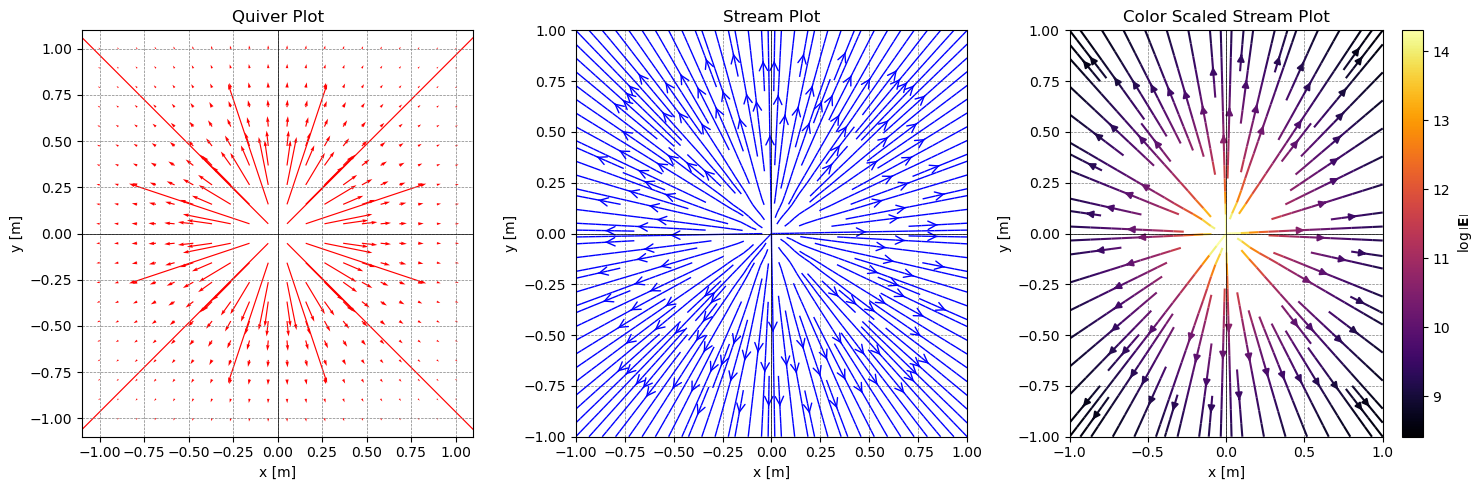
\includegraphics[keepaspectratio,alt={png}]{../images/activity-efields_activity-efields_tmp_5_0.png}}
\caption{png}
\end{figure}

\paragraph{Negative Point Charge at the
Origin}\label{negative-point-charge-at-the-origin}

\begin{Shaded}
\begin{Highlighting}[]
\NormalTok{x }\OperatorTok{=}\NormalTok{ np.linspace(}\OperatorTok{{-}}\DecValTok{1}\NormalTok{, }\DecValTok{1}\NormalTok{, }\DecValTok{20}\NormalTok{)}
\NormalTok{y }\OperatorTok{=}\NormalTok{ np.linspace(}\OperatorTok{{-}}\DecValTok{1}\NormalTok{, }\DecValTok{1}\NormalTok{, }\DecValTok{20}\NormalTok{)}
\NormalTok{X, Y }\OperatorTok{=}\NormalTok{ np.meshgrid(x, y)}

\CommentTok{\#\# A negative point charge}
\NormalTok{charge }\OperatorTok{=} \OperatorTok{{-}}\FloatTok{1e{-}6}  \CommentTok{\# C}

\NormalTok{E\_x, E\_y }\OperatorTok{=}\NormalTok{ electric\_field(charge, X, Y)}
\NormalTok{plot\_electric\_field(X, Y, E\_x, E\_y)}
\end{Highlighting}
\end{Shaded}

\begin{figure}
\centering
\pandocbounded{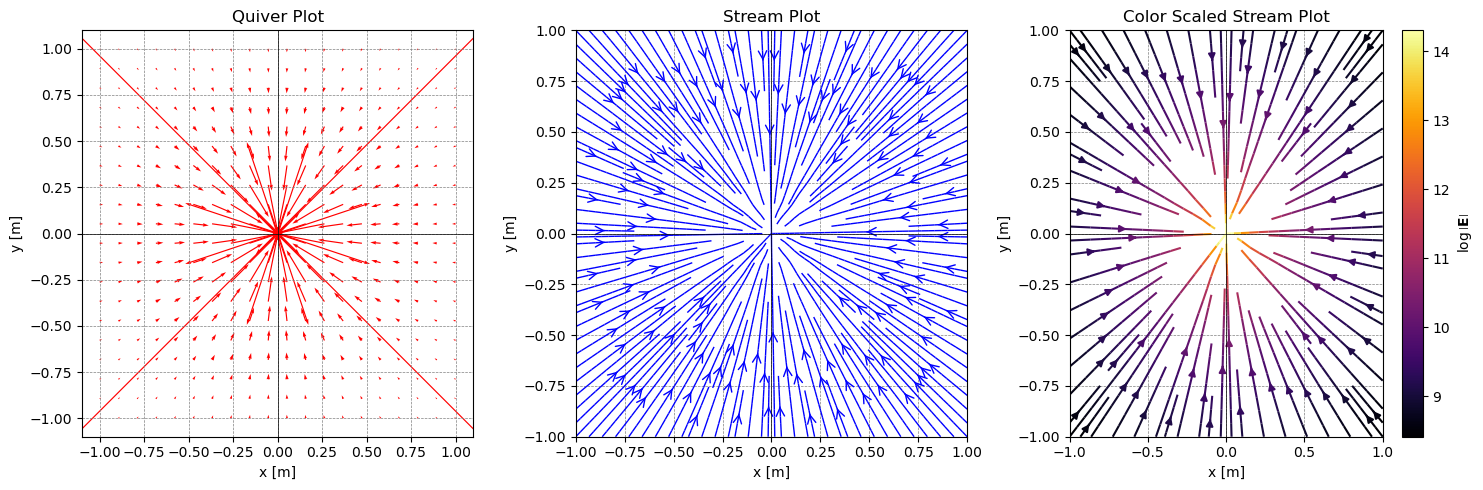
\includegraphics[keepaspectratio,alt={png}]{../images/activity-efields_activity-efields_tmp_7_0.png}}
\caption{png}
\end{figure}

\subsubsection{The electric dipole}\label{the-electric-dipole}

Now we can use these functions to place charges where we like and
compute the total field. Below, we placed two oppositely signed charges
to illustrate the field of an
\href{https://en.wikipedia.org/wiki/Electric_dipole_moment}{electric
dipole}. While not every distribution has an electric dipole moment,
many do; especially those in water (as it's a polar molecule).

\begin{Shaded}
\begin{Highlighting}[]
\NormalTok{x }\OperatorTok{=}\NormalTok{ np.linspace(}\OperatorTok{{-}}\DecValTok{1}\NormalTok{, }\DecValTok{1}\NormalTok{, }\DecValTok{20}\NormalTok{)}
\NormalTok{y }\OperatorTok{=}\NormalTok{ np.linspace(}\OperatorTok{{-}}\DecValTok{1}\NormalTok{, }\DecValTok{1}\NormalTok{, }\DecValTok{20}\NormalTok{)}
\NormalTok{X, Y }\OperatorTok{=}\NormalTok{ np.meshgrid(x, y)}

\CommentTok{\#\# A positive point charge}
\NormalTok{charge1 }\OperatorTok{=} \FloatTok{1e{-}6}  \CommentTok{\# C}
\NormalTok{x1 }\OperatorTok{=} \OperatorTok{{-}}\FloatTok{0.5}  \CommentTok{\# m}
\NormalTok{y1 }\OperatorTok{=} \DecValTok{0}  \CommentTok{\# m}

\CommentTok{\#\# A negative point charge}
\NormalTok{charge2 }\OperatorTok{=} \OperatorTok{{-}}\FloatTok{1e{-}6}  \CommentTok{\# C}
\NormalTok{x2 }\OperatorTok{=} \FloatTok{0.5}  \CommentTok{\# m}
\NormalTok{y2 }\OperatorTok{=} \DecValTok{0}  \CommentTok{\# m}

\NormalTok{E\_1\_x, E\_1\_y }\OperatorTok{=}\NormalTok{ electric\_field(charge1, X, Y, x1, y1)}
\NormalTok{E\_2\_x, E\_2\_y }\OperatorTok{=}\NormalTok{ electric\_field(charge2, X, Y, x2, y2)}


\CommentTok{\#\# Find the net electric field in each direction}
\NormalTok{E\_T\_x }\OperatorTok{=}\NormalTok{ E\_1\_x }\OperatorTok{+}\NormalTok{ E\_2\_x}
\NormalTok{E\_T\_y }\OperatorTok{=}\NormalTok{ E\_1\_y }\OperatorTok{+}\NormalTok{ E\_2\_y}

\NormalTok{plot\_electric\_field(X, Y, E\_T\_x, E\_T\_y)}
\end{Highlighting}
\end{Shaded}

\begin{figure}
\centering
\pandocbounded{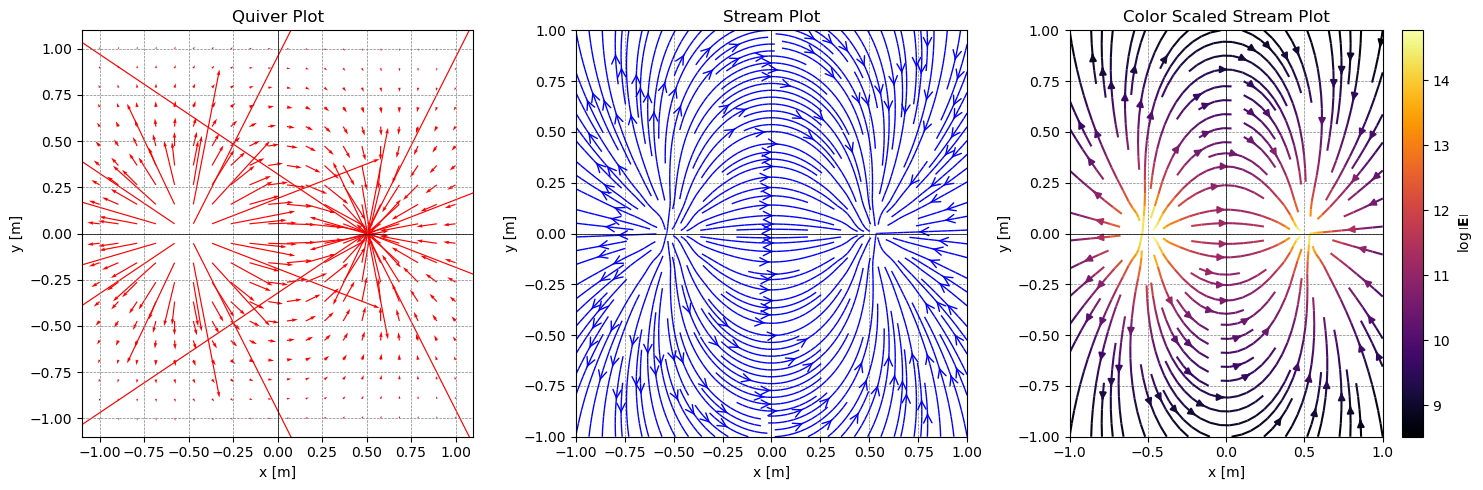
\includegraphics[keepaspectratio,alt={png}]{../images/activity-efields_activity-efields_tmp_9_0.png}}
\caption{png}
\end{figure}

\subsubsection{Quadrupole}\label{quadrupole}

We will end this game with a list of charges that we can iterate
through. This will help you develop more complicated distributions of
charges.

Below, we have a
\href{https://en.wikipedia.org/wiki/Quadrupole}{quadrupole}. You can
change the charges and their locations to see how the field changes.
Your activity below is to develop several situations and see how the
field changes and consider the symmetry of the field. For this we will
make a \href{https://docs.python.org/3/tutorial/classes.html}{Python
class} for the charges. This will allow us to create a list of charges
and iterate through them. This is showing an advantage of using aspects
of
\href{https://en.wikipedia.org/wiki/Object-oriented_programming}{object
oriented programming}.

\begin{Shaded}
\begin{Highlighting}[]
\KeywordTok{class}\NormalTok{ Charge:}
    \KeywordTok{def} \FunctionTok{\_\_init\_\_}\NormalTok{(}\VariableTok{self}\NormalTok{, q, x, y):}
        \VariableTok{self}\NormalTok{.q }\OperatorTok{=}\NormalTok{ q  }\CommentTok{\# charge value}
        \VariableTok{self}\NormalTok{.x }\OperatorTok{=}\NormalTok{ x  }\CommentTok{\# x{-}coordinate}
        \VariableTok{self}\NormalTok{.y }\OperatorTok{=}\NormalTok{ y  }\CommentTok{\# y{-}coordinate}

\CommentTok{\# Creating instances of Charge class}
\NormalTok{charge1 }\OperatorTok{=}\NormalTok{ Charge(}\FloatTok{1e{-}6}\NormalTok{, }\OperatorTok{{-}}\DecValTok{1}\NormalTok{, }\DecValTok{1}\NormalTok{)  }\CommentTok{\# e.g. Charge of 1 μC at (0, 0)}
\NormalTok{charge2 }\OperatorTok{=}\NormalTok{ Charge(}\OperatorTok{{-}}\FloatTok{1e{-}6}\NormalTok{, }\DecValTok{1}\NormalTok{, }\DecValTok{1}\NormalTok{)  }\CommentTok{\# e.g. Charge of {-}1 μC at (1, 0)}
\NormalTok{charge3 }\OperatorTok{=}\NormalTok{ Charge(}\FloatTok{1e{-}6}\NormalTok{, }\DecValTok{1}\NormalTok{, }\OperatorTok{{-}}\DecValTok{1}\NormalTok{)  }\CommentTok{\# e.g. Charge of 1 μC at (0, 1)}
\NormalTok{charge4 }\OperatorTok{=}\NormalTok{ Charge(}\OperatorTok{{-}}\FloatTok{1e{-}6}\NormalTok{, }\OperatorTok{{-}}\DecValTok{1}\NormalTok{, }\OperatorTok{{-}}\DecValTok{1}\NormalTok{)  }\CommentTok{\# e.g. Charge of {-}1 μC at (1, 1)}

\CommentTok{\# Storing instances in a list}
\NormalTok{charges }\OperatorTok{=}\NormalTok{ [charge1, charge2, charge3, charge4]}

\CommentTok{\# Iterating over the list of charges}
\ControlFlowTok{for}\NormalTok{ charge }\KeywordTok{in}\NormalTok{ charges:}
    \BuiltInTok{print}\NormalTok{(}\SpecialStringTok{f"Charge: }\SpecialCharTok{\{}\NormalTok{charge}\SpecialCharTok{.}\NormalTok{q}\SpecialCharTok{\}}\SpecialStringTok{ C, Location: (}\SpecialCharTok{\{}\NormalTok{charge}\SpecialCharTok{.}\NormalTok{x}\SpecialCharTok{\}}\SpecialStringTok{, }\SpecialCharTok{\{}\NormalTok{charge}\SpecialCharTok{.}\NormalTok{y}\SpecialCharTok{\}}\SpecialStringTok{)"}\NormalTok{)}
\end{Highlighting}
\end{Shaded}

\begin{verbatim}
Charge: 1e-06 C, Location: (-1, 1)
Charge: -1e-06 C, Location: (1, 1)
Charge: 1e-06 C, Location: (1, -1)
Charge: -1e-06 C, Location: (-1, -1)
\end{verbatim}

\begin{Shaded}
\begin{Highlighting}[]
\CommentTok{\#\# Set up the space again}
\NormalTok{x }\OperatorTok{=}\NormalTok{ np.linspace(}\OperatorTok{{-}}\DecValTok{2}\NormalTok{, }\DecValTok{2}\NormalTok{, }\DecValTok{40}\NormalTok{)}
\NormalTok{y }\OperatorTok{=}\NormalTok{ np.linspace(}\OperatorTok{{-}}\DecValTok{2}\NormalTok{, }\DecValTok{2}\NormalTok{, }\DecValTok{40}\NormalTok{)}
\NormalTok{X, Y }\OperatorTok{=}\NormalTok{ np.meshgrid(x, y)}

\CommentTok{\#\# Set the total electric field to zero}
\NormalTok{E\_T\_x }\OperatorTok{=}\NormalTok{ np.zeros\_like(X)}
\NormalTok{E\_T\_y }\OperatorTok{=}\NormalTok{ np.zeros\_like(Y)}

\CommentTok{\#\# Calculate the electric field due to each charge}
\ControlFlowTok{for}\NormalTok{ charge }\KeywordTok{in}\NormalTok{ charges:}
\NormalTok{    E\_x, E\_y }\OperatorTok{=}\NormalTok{ electric\_field(charge.q, X, Y, charge.x, charge.y)}
\NormalTok{    E\_T\_x }\OperatorTok{+=}\NormalTok{ E\_x}
\NormalTok{    E\_T\_y }\OperatorTok{+=}\NormalTok{ E\_y}

\NormalTok{plot\_electric\_field(X, Y, E\_T\_x, E\_T\_y)}
\end{Highlighting}
\end{Shaded}

\begin{figure}
\centering
\pandocbounded{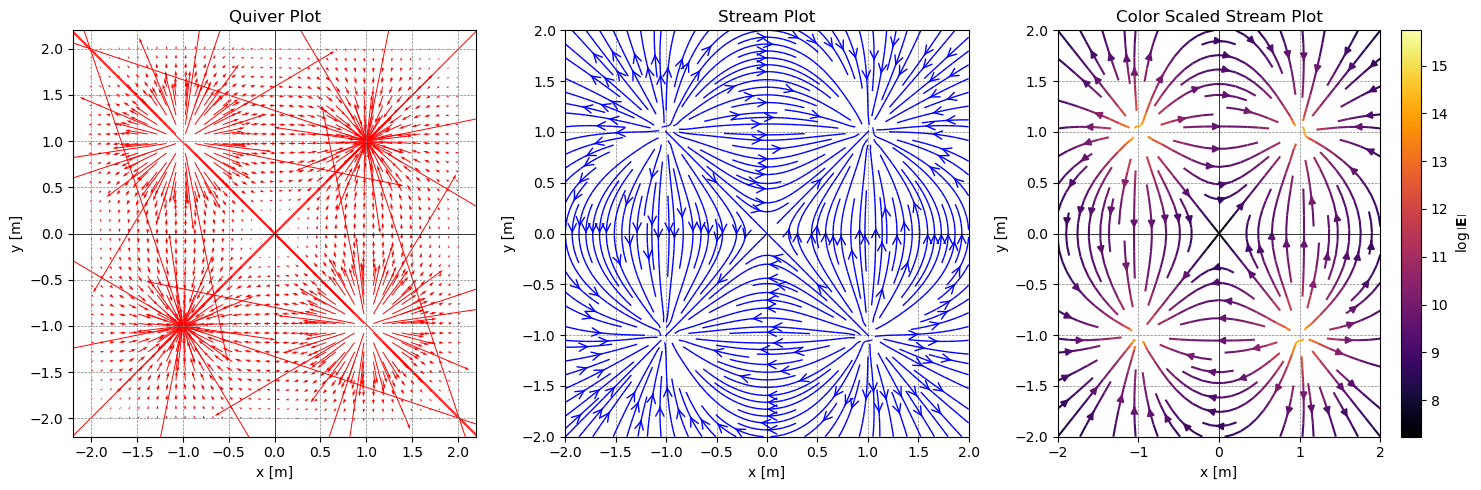
\includegraphics[keepaspectratio,alt={png}]{../images/activity-efields_activity-efields_tmp_12_0.png}}
\caption{png}
\end{figure}

\textbf{✅ Do this}

Now that we have built up some visualization codes. Let's make use of
them. Create the following graphics and answer the following questions.

\begin{itemize}
\tightlist
\item
  Create a uniform line of charges. Make sure to include enough charges
  so that the field looks smooth. What is the symmetry of this
  situation. Where is the electric field constant (if at all)? Where is
  the electric field zero (if at all)?
\item
  What if the line of charges varying their strength like a sinusoidal
  function?
\item
  Create a circle of charges (like a ring). Is there any symmetry to
  this situation? Where is the electric field zero? How close does your
  calculation get to zero? What makes the calculation better or worse?
\item
  Create a small locus of charges of different sizes and signs, but make
  sure the net charge is non-zero. How close do the charges need to be
  (or how far away do you need to be) for the field to look like a point
  charge field? What is the symmetry of this situation (or approximately
  so)? Where is the electric field zero (if at all)?
\end{itemize}

\paragraph{Uniform line of charges}\label{uniform-line-of-charges}

\begin{Shaded}
\begin{Highlighting}[]
\CommentTok{\#\# Set up the space again}
\NormalTok{size }\OperatorTok{=} \DecValTok{2}
\NormalTok{step }\OperatorTok{=} \DecValTok{40}

\NormalTok{x }\OperatorTok{=}\NormalTok{ np.linspace(}\OperatorTok{{-}}\NormalTok{size, size, step)}
\NormalTok{y }\OperatorTok{=}\NormalTok{ np.linspace(}\OperatorTok{{-}}\NormalTok{size, size, step)}
\NormalTok{X, Y }\OperatorTok{=}\NormalTok{ np.meshgrid(x, y)}

\NormalTok{N }\OperatorTok{=} \DecValTok{100}  \CommentTok{\# Number of charges}
\NormalTok{charges }\OperatorTok{=}\NormalTok{ []}
\ControlFlowTok{for}\NormalTok{ i }\KeywordTok{in} \BuiltInTok{range}\NormalTok{(N):}
\NormalTok{    q }\OperatorTok{=} \FloatTok{1e{-}6}  \CommentTok{\# Charge Value}
\NormalTok{    x }\OperatorTok{=}\NormalTok{ i}\OperatorTok{*}\NormalTok{(}\DecValTok{2}\OperatorTok{*}\NormalTok{size)}\OperatorTok{/}\NormalTok{(N}\OperatorTok{{-}}\DecValTok{1}\NormalTok{) }\OperatorTok{{-}}\NormalTok{ size  }\CommentTok{\# Spread the charges out}
\NormalTok{    y }\OperatorTok{=} \DecValTok{0}  \CommentTok{\# everything on the x{-}axis}
\NormalTok{    charges.append(Charge(q, x, y))  }\CommentTok{\# Add the charge to the list of charges}

\CommentTok{\#\# Set the total electric field to zero}
\NormalTok{E\_T\_x }\OperatorTok{=}\NormalTok{ np.zeros\_like(X)}
\NormalTok{E\_T\_y }\OperatorTok{=}\NormalTok{ np.zeros\_like(Y)}

\CommentTok{\#\# Calculate the electric field due to each charge}
\ControlFlowTok{for}\NormalTok{ charge }\KeywordTok{in}\NormalTok{ charges:}
\NormalTok{    E\_x, E\_y }\OperatorTok{=}\NormalTok{ electric\_field(charge.q, X, Y, charge.x, charge.y)}
\NormalTok{    E\_T\_x }\OperatorTok{+=}\NormalTok{ E\_x}
\NormalTok{    E\_T\_y }\OperatorTok{+=}\NormalTok{ E\_y}

\NormalTok{plot\_electric\_field(X, Y, E\_T\_x, E\_T\_y)}
\end{Highlighting}
\end{Shaded}

\begin{figure}
\centering
\pandocbounded{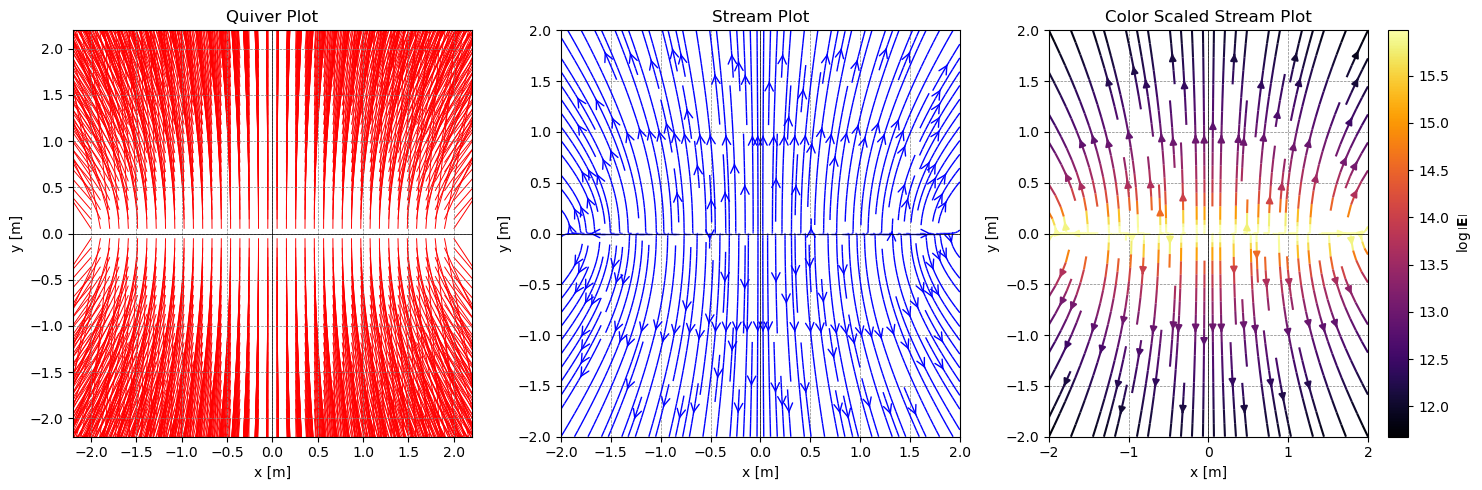
\includegraphics[keepaspectratio,alt={png}]{../images/activity-efields_activity-efields_tmp_15_0.png}}
\caption{png}
\end{figure}

\paragraph{Sinusoidal line of charges}\label{sinusoidal-line-of-charges}

\begin{Shaded}
\begin{Highlighting}[]
\CommentTok{\#\# Set up the space again}
\NormalTok{size }\OperatorTok{=} \DecValTok{2}
\NormalTok{step }\OperatorTok{=} \DecValTok{100}

\NormalTok{x }\OperatorTok{=}\NormalTok{ np.linspace(}\OperatorTok{{-}}\NormalTok{size, size, step)}
\NormalTok{y }\OperatorTok{=}\NormalTok{ np.linspace(}\OperatorTok{{-}}\NormalTok{size, size, step)}
\NormalTok{X, Y }\OperatorTok{=}\NormalTok{ np.meshgrid(x, y)}

\NormalTok{N }\OperatorTok{=} \DecValTok{600}  \CommentTok{\# Number of charges}
\NormalTok{charges }\OperatorTok{=}\NormalTok{ []}
\ControlFlowTok{for}\NormalTok{ i }\KeywordTok{in} \BuiltInTok{range}\NormalTok{(N):}
\NormalTok{    x }\OperatorTok{=}\NormalTok{ i}\OperatorTok{*}\NormalTok{(}\DecValTok{2}\OperatorTok{*}\NormalTok{size)}\OperatorTok{/}\NormalTok{(N}\OperatorTok{{-}}\DecValTok{1}\NormalTok{) }\OperatorTok{{-}}\NormalTok{ size  }\CommentTok{\# Spread the charges out}
\NormalTok{    y }\OperatorTok{=} \DecValTok{0}  \CommentTok{\# everything on the x{-}axis}
    
\NormalTok{    q }\OperatorTok{=} \FloatTok{1e{-}6}\OperatorTok{*}\NormalTok{np.sin(}\DecValTok{30}\OperatorTok{*}\NormalTok{x}\OperatorTok{/}\NormalTok{(size))  }\CommentTok{\# Charge Value}
    
\NormalTok{    charges.append(Charge(q, x, y))  }\CommentTok{\# Add the charge to the list of charges}

\CommentTok{\#\# Set the total electric field to zero}
\NormalTok{E\_T\_x }\OperatorTok{=}\NormalTok{ np.zeros\_like(X)}
\NormalTok{E\_T\_y }\OperatorTok{=}\NormalTok{ np.zeros\_like(Y)}

\CommentTok{\#\# Calculate the electric field due to each charge}
\ControlFlowTok{for}\NormalTok{ charge }\KeywordTok{in}\NormalTok{ charges:}
\NormalTok{    E\_x, E\_y }\OperatorTok{=}\NormalTok{ electric\_field(charge.q, X, Y, charge.x, charge.y)}
\NormalTok{    E\_T\_x }\OperatorTok{+=}\NormalTok{ E\_x}
\NormalTok{    E\_T\_y }\OperatorTok{+=}\NormalTok{ E\_y}

\NormalTok{plot\_electric\_field(X, Y, E\_T\_x, E\_T\_y)}
\end{Highlighting}
\end{Shaded}

\begin{figure}
\centering
\pandocbounded{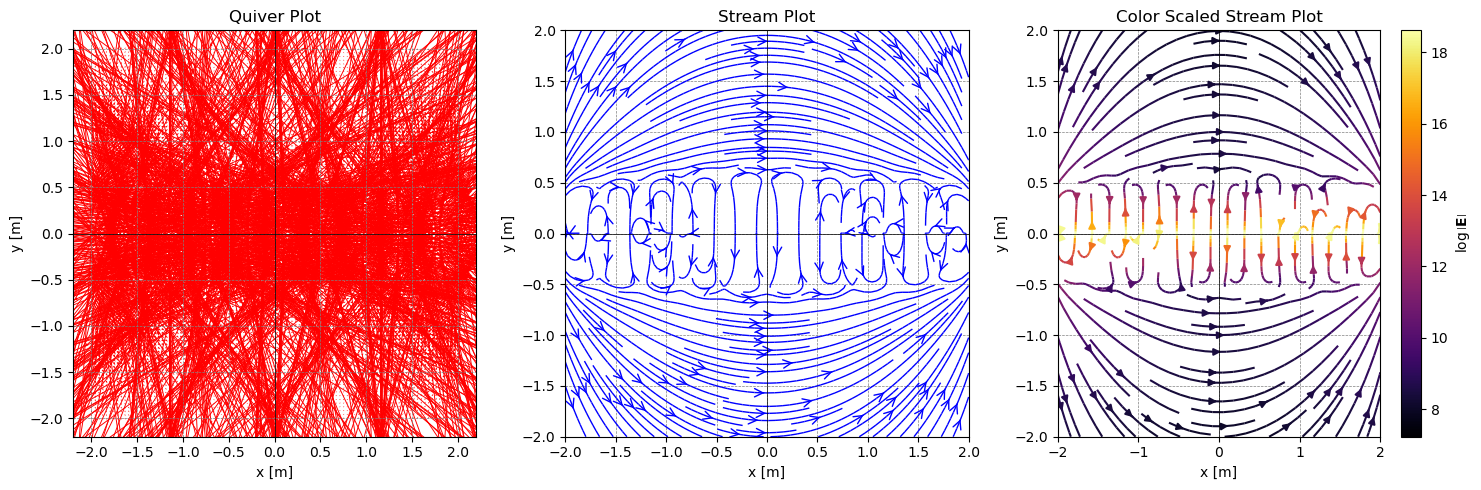
\includegraphics[keepaspectratio,alt={png}]{../images/activity-efields_activity-efields_tmp_17_0.png}}
\caption{png}
\end{figure}

\paragraph{Circle of charges}\label{circle-of-charges}

\begin{Shaded}
\begin{Highlighting}[]
\CommentTok{\#\# Set up the space again}
\NormalTok{size }\OperatorTok{=} \DecValTok{2}
\NormalTok{step }\OperatorTok{=} \DecValTok{100}
\NormalTok{R }\OperatorTok{=}\NormalTok{ size}\OperatorTok{/}\DecValTok{2}

\NormalTok{x }\OperatorTok{=}\NormalTok{ np.linspace(}\OperatorTok{{-}}\NormalTok{size, size, step)}
\NormalTok{y }\OperatorTok{=}\NormalTok{ np.linspace(}\OperatorTok{{-}}\NormalTok{size, size, step)}
\NormalTok{X, Y }\OperatorTok{=}\NormalTok{ np.meshgrid(x, y)}

\NormalTok{N }\OperatorTok{=} \DecValTok{360}  \CommentTok{\# Number of charges}
\NormalTok{charges }\OperatorTok{=}\NormalTok{ []}
\ControlFlowTok{for}\NormalTok{ i }\KeywordTok{in} \BuiltInTok{range}\NormalTok{(N):}
    
\NormalTok{    theta }\OperatorTok{=}\NormalTok{ i}\OperatorTok{*}\NormalTok{(}\DecValTok{2}\OperatorTok{*}\NormalTok{np.pi)}\OperatorTok{/}\NormalTok{(N}\OperatorTok{{-}}\DecValTok{1}\NormalTok{)  }\CommentTok{\# Spread the charges out}
\NormalTok{    x }\OperatorTok{=}\NormalTok{ R}\OperatorTok{*}\NormalTok{np.cos(theta)}
\NormalTok{    y }\OperatorTok{=}\NormalTok{ R}\OperatorTok{*}\NormalTok{np.sin(theta)}
    
\NormalTok{    q }\OperatorTok{=} \FloatTok{1e{-}6}  \CommentTok{\# Charge Value}
    
\NormalTok{    charges.append(Charge(q, x, y))  }\CommentTok{\# Add the charge to the list of charges}

\CommentTok{\#\# Set the total electric field to zero}
\NormalTok{E\_T\_x }\OperatorTok{=}\NormalTok{ np.zeros\_like(X)}
\NormalTok{E\_T\_y }\OperatorTok{=}\NormalTok{ np.zeros\_like(Y)}

\CommentTok{\#\# Calculate the electric field due to each charge}
\ControlFlowTok{for}\NormalTok{ charge }\KeywordTok{in}\NormalTok{ charges:}
\NormalTok{    E\_x, E\_y }\OperatorTok{=}\NormalTok{ electric\_field(charge.q, X, Y, charge.x, charge.y)}
\NormalTok{    E\_T\_x }\OperatorTok{+=}\NormalTok{ E\_x}
\NormalTok{    E\_T\_y }\OperatorTok{+=}\NormalTok{ E\_y}

\NormalTok{plot\_electric\_field(X, Y, E\_T\_x, E\_T\_y)}
    
\end{Highlighting}
\end{Shaded}

\begin{figure}
\centering
\pandocbounded{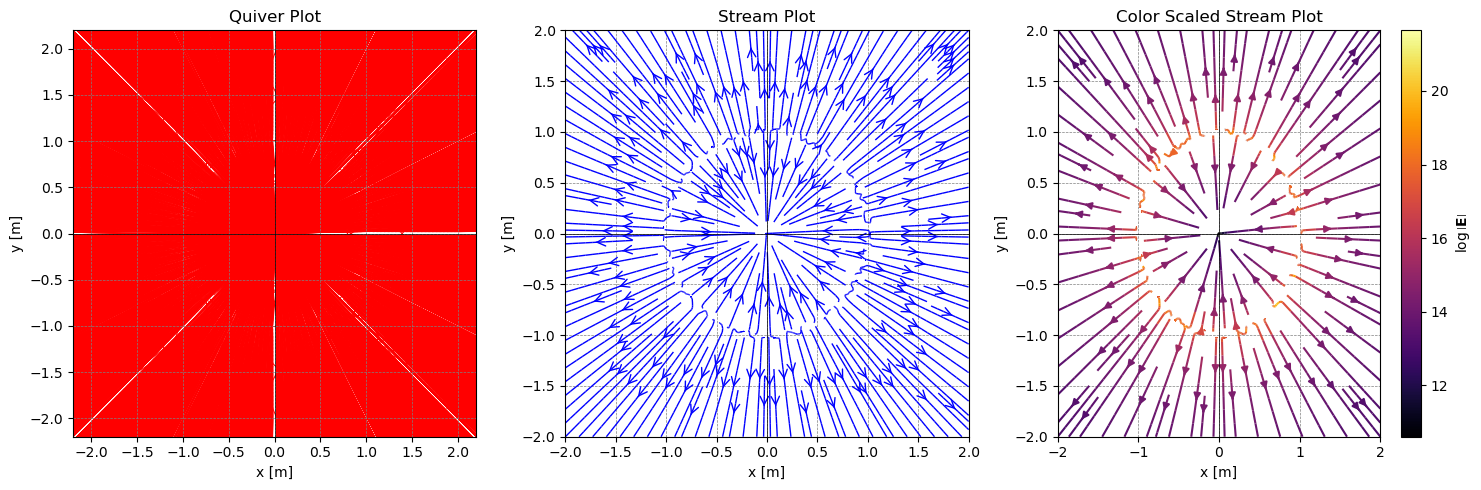
\includegraphics[keepaspectratio,alt={png}]{../images/activity-efields_activity-efields_tmp_19_0.png}}
\caption{png}
\end{figure}

\paragraph{Small Locus of Random
Charges}\label{small-locus-of-random-charges}

\begin{Shaded}
\begin{Highlighting}[]
\CommentTok{\#\# Set up the space again}
\NormalTok{size }\OperatorTok{=} \DecValTok{2}
\NormalTok{step }\OperatorTok{=} \DecValTok{100}
\NormalTok{R }\OperatorTok{=}\NormalTok{ size}\OperatorTok{/}\DecValTok{2}
\NormalTok{scale }\OperatorTok{=} \FloatTok{1e{-}3} \CommentTok{\#smaller scale means charges are closer to the origin}

\NormalTok{x }\OperatorTok{=}\NormalTok{ np.linspace(}\OperatorTok{{-}}\NormalTok{size, size, step)}
\NormalTok{y }\OperatorTok{=}\NormalTok{ np.linspace(}\OperatorTok{{-}}\NormalTok{size, size, step)}
\NormalTok{X, Y }\OperatorTok{=}\NormalTok{ np.meshgrid(x, y)}

\NormalTok{N }\OperatorTok{=} \DecValTok{6} \CommentTok{\# If even there\textquotesingle{}s a chance of a net charge of zero}
\NormalTok{charges }\OperatorTok{=}\NormalTok{ []}
\ControlFlowTok{for}\NormalTok{ i }\KeywordTok{in} \BuiltInTok{range}\NormalTok{(N):}
    
    \CommentTok{\#\# Random charge value}
\NormalTok{    q }\OperatorTok{=}\NormalTok{ np.random.choice([}\OperatorTok{{-}}\FloatTok{1e{-}6}\NormalTok{, }\FloatTok{1e{-}6}\NormalTok{]) }\CommentTok{\# Either a positive or negative charge}
    \CommentTok{\#\# Random x,y locations that are located close to the origin}
\NormalTok{    x }\OperatorTok{=}\NormalTok{ np.random.uniform(}\OperatorTok{{-}}\NormalTok{scale}\OperatorTok{*}\NormalTok{size, scale}\OperatorTok{*}\NormalTok{size)}
\NormalTok{    y }\OperatorTok{=}\NormalTok{ np.random.uniform(}\OperatorTok{{-}}\NormalTok{scale}\OperatorTok{*}\NormalTok{size, scale}\OperatorTok{*}\NormalTok{size)}
    
\NormalTok{    charges.append(Charge(q, x, y))  }\CommentTok{\# Add the charge to the list of charges}

\CommentTok{\#\# Set the total electric field to zero}
\NormalTok{E\_T\_x }\OperatorTok{=}\NormalTok{ np.zeros\_like(X)}
\NormalTok{E\_T\_y }\OperatorTok{=}\NormalTok{ np.zeros\_like(Y)}

\CommentTok{\#\# Calculate the electric field due to each charge}
\ControlFlowTok{for}\NormalTok{ charge }\KeywordTok{in}\NormalTok{ charges:}
\NormalTok{    E\_x, E\_y }\OperatorTok{=}\NormalTok{ electric\_field(charge.q, X, Y, charge.x, charge.y)}
\NormalTok{    E\_T\_x }\OperatorTok{+=}\NormalTok{ E\_x}
\NormalTok{    E\_T\_y }\OperatorTok{+=}\NormalTok{ E\_y}

\NormalTok{plot\_electric\_field(X, Y, E\_T\_x, E\_T\_y)}

\NormalTok{total\_charge }\OperatorTok{=} \DecValTok{0}

\ControlFlowTok{for}\NormalTok{ charge }\KeywordTok{in}\NormalTok{ charges:}
    \BuiltInTok{print}\NormalTok{(}\SpecialStringTok{f"Charge: }\SpecialCharTok{\{}\NormalTok{charge}\SpecialCharTok{.}\NormalTok{q}\SpecialCharTok{\}}\SpecialStringTok{ C, Location: (}\SpecialCharTok{\{}\NormalTok{charge}\SpecialCharTok{.}\NormalTok{x}\SpecialCharTok{\}}\SpecialStringTok{, }\SpecialCharTok{\{}\NormalTok{charge}\SpecialCharTok{.}\NormalTok{y}\SpecialCharTok{\}}\SpecialStringTok{)"}\NormalTok{)}
\NormalTok{    total\_charge }\OperatorTok{+=}\NormalTok{ charge.q}
    
\BuiltInTok{print}\NormalTok{(}\SpecialStringTok{f"Total Charge: }\SpecialCharTok{\{}\NormalTok{total\_charge}\SpecialCharTok{\}}\SpecialStringTok{ C"}\NormalTok{)}
\end{Highlighting}
\end{Shaded}

\begin{figure}
\centering
\pandocbounded{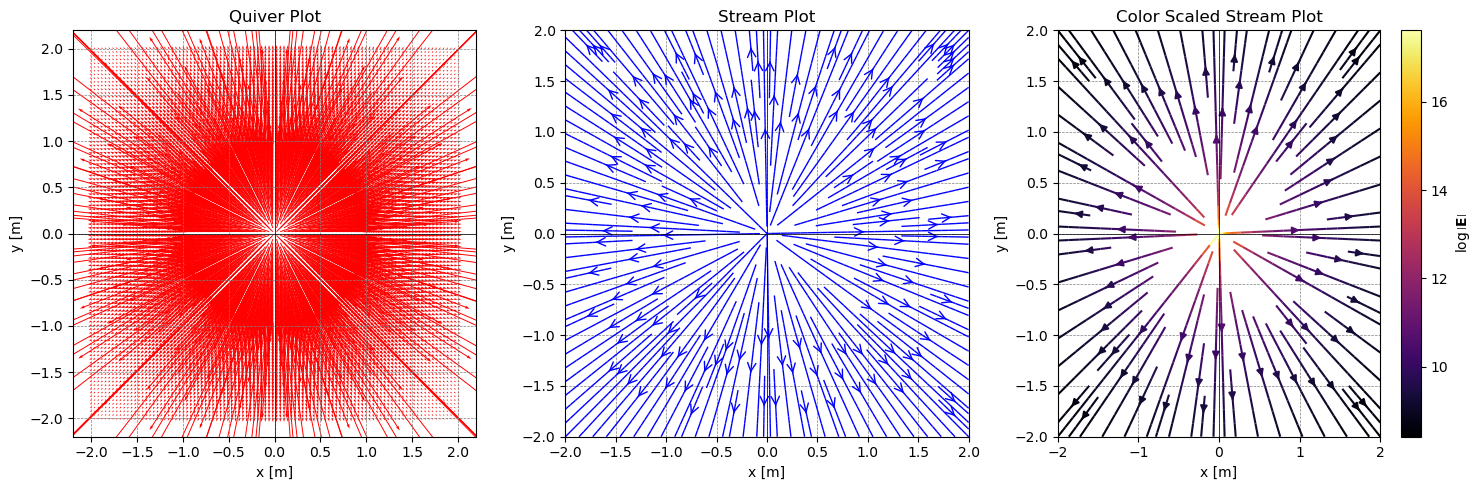
\includegraphics[keepaspectratio,alt={png}]{../images/activity-efields_activity-efields_tmp_21_0.png}}
\caption{png}
\end{figure}

\begin{verbatim}
Charge: 1e-06 C, Location: (-0.0012184532929861245, -0.0004979964164912648)
Charge: 1e-06 C, Location: (0.00048390202162626635, 0.0014723630957774528)
Charge: 1e-06 C, Location: (-0.0006583745072223969, -0.00044763882490302283)
Charge: 1e-06 C, Location: (0.0011431645429140196, 0.001931463822718301)
Charge: 1e-06 C, Location: (-5.60897369906103e-05, -0.0003944506192641625)
Charge: -1e-06 C, Location: (-0.0011296991527068485, 0.0017233177048307227)
Total Charge: 4e-06 C
\end{verbatim}

\subsection{Gauss's Law}\label{gausss-law}

Clearly Coulomb's Law gives us a prescription to solve most problems and
serves as the basis for generic approaches to solving these problems.
However, we can use the
\href{https://en.wikipedia.org/wiki/Divergence_theorem}{divergence
theorem} with the first of the electrostatic equations above. This will
convert this equation into a tool for solving highly symmetric problems.

\[\int \int \int \nabla \cdot \mathbf{E}\;dV = \int \int \int \dfrac{\rho}{\epsilon_0} \;dV\]

The left hand side can be rewritten as:

\[\int \int \int \nabla \cdot \mathbf{E}\;dV = \iint \mathbf{E} \cdot d\mathbf{A}\]

where \(d\mathbf{A}\) is an infinitesimal area element that has a vector
direction. It points outward from the surface (normal to the local
surface). We use this to write
\href{https://en.wikipedia.org/wiki/Gauss\%27s_law}{Gauss's Law} for the
electric field:

\[\iint \mathbf{E} \cdot d\mathbf{A} = \int \int \int \dfrac{\rho}{\epsilon_0}\;dV\]

Notice that this expression is always true, but it almost never useful
for solving problems in general. The electric flux is often easily
calculated considering the total enclosed charge:

\[\Phi_E = \int \int \int \dfrac{\rho}{\epsilon_0}\;dV = \dfrac{Q_{enc}}{\epsilon_0}\]

However, using that measure of the total electric flux to find the field
is only possible in highly symmetric situations. For example, if we have
a spherical charge distribution \(\rho(r)\), we can use Gauss's Law to
find the electric field at any point outside the sphere. Below, is a
figure of a cylindrical charge distribution. We can use Gauss's Law to
find the electric field at any point outside the cylinder because the
charge per unit length is constant.

\begin{figure}
\centering
\pandocbounded{\includegraphics[keepaspectratio,alt={Gaussian Cylinder}]{http://hyperphysics.phy-astr.gsu.edu/hbase/electric/imgele/gaucyl2.png}}
\caption{Gaussian Cylinder}
\end{figure}

\subsubsection{A charged cylinder}\label{a-charged-cylinder}

\textbf{✅ Do this}

Consider a long and thin plastic cylinder with a radius of \(R_0\) and
length \(L\), such that \(L>>R_0\). The cylinder has a charge
distribution that varies with radius \(\rho(r) = cr^2\), where \(c\) is
a positive constant. Find the electric field inside and outside the
cylinder using Gauss's Law.

\begin{itemize}
\tightlist
\item
  Sketch the situation. What are the units of \(c\)?
\item
  Prove to yourself and your group that you can use Gauss's Law to find
  the electric field inside and outside the cylinder (why? what
  assumptions are you making?)
\item
  Compute the electric field and graph it's magnitude
  \(|\mathbf{E}(r)|\) as a function of \(r\) for \(r \in [0,4R_0]\).
\end{itemize}

\subsubsection{Invent a planar problem}\label{invent-a-planar-problem}

\textbf{✅ Do this}

It is very common to show that the electric field on a planar surface is
given by:

\[\mathbf{E} = \dfrac{\sigma}{2\epsilon_0}\]

where \(\sigma\) is the charge density on the surface (typically,
\(Q/A\)). We can use Gauss's Law to find the electric field due to a
charged plane. But, we want you to invent a problem for a thick plane of
charge that has a varying charge density that depends on the distance
from the center of the plane.

\begin{enumerate}
\def\labelenumi{\arabic{enumi}.}
\tightlist
\item
  Invent this problem and sketch it. Note here:
  \(\rho(\mathbf{r}) = \rho(z)\) will still allow you to use Gauss's
  Law.
\item
  Solve for the electric field using Gauss's Law inside and outside the
  thick plane.
\end{enumerate}

\subsection{Numerical Superposition - Coulomb's
Law}\label{numerical-superposition---coulombs-law}

We gave you code and a class structure that lets you develop solutions
to 2D electrostatic problems. In fact, we built a simple numerical
integrator that uses superposition in 2D to solve for the electric
field. This works because the electric field obeys superposition. So we
can add up the electric field due to each charge.

\[\mathbf{E} = \sum_i \mathbf{E}_i = \sum_i \dfrac{q_i}{4\pi\epsilon_0} \dfrac{\mathbf{r} - \mathbf{r}_i}{\left|\mathbf{r} - \mathbf{r}_i\right|^3}\]

In the continuous limit (\(q \rightarrow \rho\;dV\)), this becomes an
integral that we can solve (sometimes). It depends on our ability to
express the results in integrable functions:

\[\mathbf{E} = \int \int \int \dfrac{\rho(\mathbf{r}')}{4\pi\epsilon_0} \dfrac{\mathbf{r} - \mathbf{r}'}{\left|\mathbf{r} - \mathbf{r}'\right|^3} dV'\]

However, the scheme to numerically integrate this expression to find the
field follows this prescription. And as long as we avoid singularities
and the sources are compact (locally distributed), we simply add the
contributions numerically. We can use smaller and smaller chunks of the
continuous distribution to get better approximations.

\[\mathbf{E} \approx \sum_i \dfrac{\rho(\mathbf{r}_i)}{4\pi\epsilon_0} \dfrac{\mathbf{r} - \mathbf{r}_i}{\left|\mathbf{r} - \mathbf{r}_i\right|^3} \Delta V_i  = \sum_i \mathbf{E_{pt}}_i \]

where \(\mathbf{E_{pt}}_i\) is electric field of the ith point charge
with charge \(\rho(\mathbf{r}_i)\Delta V_i = q_i\). That is effectively
what our 2D electric field visualization code does. It is a numerical
integrator that uses superposition to find the electric field.

\textbf{✅ Do this}

\begin{itemize}
\tightlist
\item
  Abstract our code to 3D. This will be a usueful tool for you to use in
  the future.
\item
  Create known 3D distributions of charges and demonstrate you can view
  the field in 3D.

  \begin{itemize}
  \tightlist
  \item
    Note the visualizations will have to change more than the code to
    create the charges and compute their fields.
  \end{itemize}
\end{itemize}

\begin{Shaded}
\begin{Highlighting}[]
\CommentTok{\#\# Your code here}
\end{Highlighting}
\end{Shaded}
